In the previous part, we dealt with the optimization of a production plant with respect to the constraints of the bill of material in order to produce and fulfill orders from our customers. If we take a step backward however, we can regard our production plant as a sort of "black box" which turns orders into available final products. By considering only upper bounds for the production time for each order, we can study how and when to produce items without taking into accounts the details of the bill of material. This new part of the course will be dedicated to the study of production scheduling problems. The first part of this chapter will present the basic concepts of scheduling while the second part will introduce very basic rules to optimize certain objective functions which we will discuss. 

\section{General scheduling problems}

Scheduling problems are a combination of three decisions to be made at the same time, which are : 
\begin{description}
    \item[Assignment] : associating each and every task to one resource (some resources can remain unused). $\forall$ task $\tau_i$, associate one resource $R_j$ : $\tau_i \mapsto (\tau_i, R_j)$
    \item[Sequencing] : deciding a permutation among the set of tasks to be performed in that specific order. $T=\{\tau_1, ..., \tau_N\} \mapsto (\tau_1, \tau_5, \tau_3, ..., \tau_2)$. $\forall (\tau_i, \tau_j)\in T, t_{\tau_i} < t_{\tau_j}$ or $t_{\tau_j} < t_{\tau_i}$.
    \item[Time tabling] : choosing explicitely the time at which each task should begin its processing. 
\end{description}
Clearly, an optimal solution for the scheduling problem has to simultaneously take into account these three characteristics. However, heuristic approaches often build up a solution incrementaly taking these "steps" seperately. 

In our case, the number of resources (number of machies) is just one since the only "resource" we have is the abstracted production plant. 

When dealing with scheduling problem, we often introduce variables representing the completion time $C_i$ of one task $\tau_i$ which is the moment in time at which the task has been performed. That moment come, if possible, before a given due date $dd_i$. To characterize the fact that a task is performed too late with respect to the due date, we introduce the "lateness" function as $L_i = C_i - dd_i$ which is negative if the task is early, $0$ if the task is performed just in time and positive if the task is late. Sometimes, we also consider "tardiness" which is analogous to lateness except that early tasks are valued with $0$, it can be expressed as $T_i = \max(0, C_i - dd_i)$. Finally, we may consider as well the "tardy job" indicator $U_i$ which equals $1$ if the job $\tau_i$ is tardy and $0$ otherwise. 

In general, scheduling is an attempt to minimize an objective function taking into account every possible sequencing and every possible timetabling. We say that a cost function $J$ is "regular" if and only if $\frac{\partial J}{\partial C_i}\ge 0,\forall i$. In other words, the value of $J$ decreases when each $C_i$ decreases : the sooner the better. Thus, for that kind of cost functions, only the sequencing of the task is necessary since, following the "the sooner the better" rule, timetabling is performed by following the established sequencing without idle time between the task. 

\section{Basic rules for scheduling}

In this section, we will introduce very basic rules to solve some of the simplest scheduling problems. The examples given will all refer to figure (\ref{scheduling:table}) which shows a set of tasks with both their processing time and due dates. 

\begin{figure}[h!]
    \centering
    \begin{tabular}{|c|c|c|c|c|c|c|c|}
        \hline
         & $\tau_1$ & $\tau_2$ & $\tau_3$ & $\tau_4$ & $\tau_5$ & $\tau_6$ & $\tau_7$ \\\hline
        $t_i$ & 5 & 10 & 7 & 6 & 8 & 10 & 5\\\hline
        $dd_i$ & 20 & 100 & 50 & 40 & 30 & 35 & 55\\\hline
    \end{tabular}
    \caption{\label{scheduling:table}A set of tasks with their processing times $t_i$ and due dates $dd_i$}
\end{figure}

\subsection{Shortest Processing Time first (SPT)}

The SPT rule consists of ordering the tasks by their processing time to define the sequencing of tasks. This rule is optimal for any regular cost function. For instance, the following cost function : \[ \textrm{minimize } J = \frac{1}{N}\sum_{i=1}^N C_i \] where $N$ is the number of tasks is a regular function and the corresponding solution is represented in figure (\ref{scheduling:sol_spt}). 

\begin{figure}[h!]
    \centering
    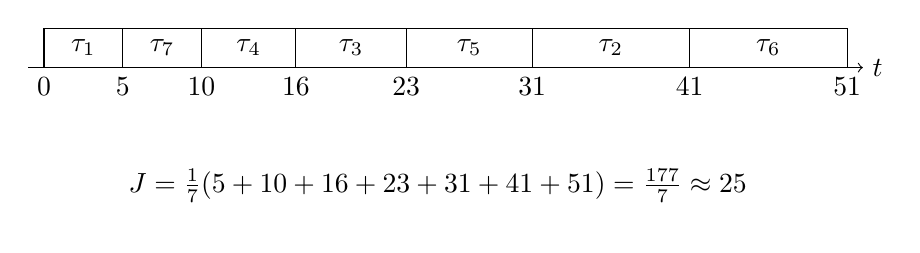
\begin{tikzpicture}[xscale=0.2]
        \draw[->] (-1,0) -- (52, 0) node[right] {$t$};

        \draw (0,0) node[below] {$0$} rectangle node {$\tau_1$} (5, .5);
        \draw (5, 0) node[below] {$5$} rectangle node {$\tau_7$} (10, .5);
        \draw (10, 0) node[below] {$10$} rectangle node {$\tau_4$} (16, .5);
        \draw (16, 0) node[below] {$16$} rectangle node {$\tau_3$} (23, .5);
        \draw (23, 0) node[below] {$23$} rectangle node {$\tau_5$} (31, .5);
        \draw (31, 0) node[below] {$31$} rectangle node {$\tau_2$} (41, .5);
        \draw (41, 0) node[below] {$41$} rectangle node {$\tau_6$} (51, .5);
        \draw (51, 0) node[below] {$51$};

        \path (-1, -1) rectangle node {$J = \frac{1}{7}(5+10+16+23+31+41+51) = \frac{177}{7} \approx 25$} (51, -2);
    \end{tikzpicture}
    \caption{\label{scheduling:sol_spt}Solution using the SPT rule for minimizing $J = \frac{1}{N}\sum_iC_i$}
\end{figure}

\subsection{Earliest Due-Date first (EDD)}

The earliest due date rule is used to minimize the maximum lateness defined as \[ \textrm{minimize } J = \max_i L_i \]
Note that this does not necessary means that one task will be late, it simply says that even the task with the maximum lateness (which can be negative in case of an early task) should be put as small as possible (which means, in case of an early task, as soon as possible). The solution of this problem with the data from figure (\ref{scheduling:table}) is represented in figure (\ref{scheduling:sol_edd}). In this case, you will notice that no tasks are late with respect to their due date and that the EDD does not allow idle time between the tasks. 

\begin{figure}[h!]
    \centering
    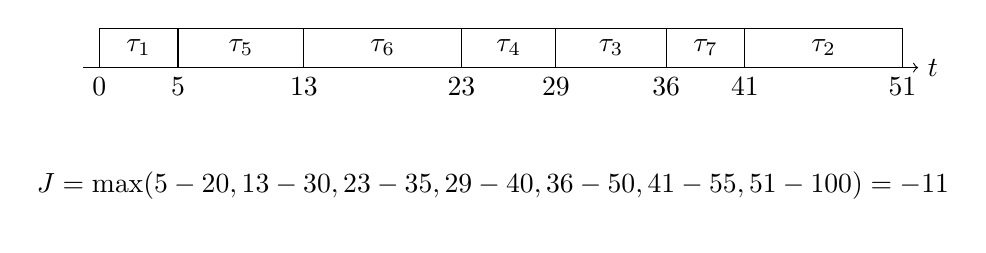
\begin{tikzpicture}[xscale=0.2]
        \draw[->] (-1,0) -- (52, 0) node[right] {$t$};

        \draw (0,0) node[below] {$0$} rectangle node {$\tau_1$} (5, .5);
        \draw (5,0) node[below] {$5$} rectangle node {$\tau_5$} (13, .5);
        \draw (13,0) node[below] {$13$} rectangle node {$\tau_6$} (23, .5);
        \draw (23,0) node[below] {$23$} rectangle node {$\tau_4$} (29, .5);
        \draw (29,0) node[below] {$29$} rectangle node {$\tau_3$} (36, .5);
        \draw (36,0) node[below] {$36$} rectangle node {$\tau_7$} (41, .5);
        \draw (41,0) node[below] {$41$} rectangle node {$\tau_2$} (51, .5);
        \draw (51, 0) node[below] {$51$};

        \path (-1, -1) rectangle node {$J = \max(5-20, 13-30, 23-35, 29-40, 36-50, 41-55, 51-100) = -11$} (51, -2);

    \end{tikzpicture}
    \caption{\label{scheduling:sol_edd}Solution using the EDD rule for minimizing $J = \max L_i$}
\end{figure}

\subsection{Moore algorithm}
